% Brain MRI: include all paper tables as PNG figures
% Requires: \usepackage{graphicx}
% Usage: % Brain MRI: include all paper tables as PNG figures
% Requires: \usepackage{graphicx}
% Usage: % Brain MRI: include all paper tables as PNG figures
% Requires: \usepackage{graphicx}
% Usage: % Brain MRI: include all paper tables as PNG figures
% Requires: \usepackage{graphicx}
% Usage: \input{paper_tables/brain_tumor_mri/all_tables_figures.tex}

\begin{figure}[htbp]
  \centering
  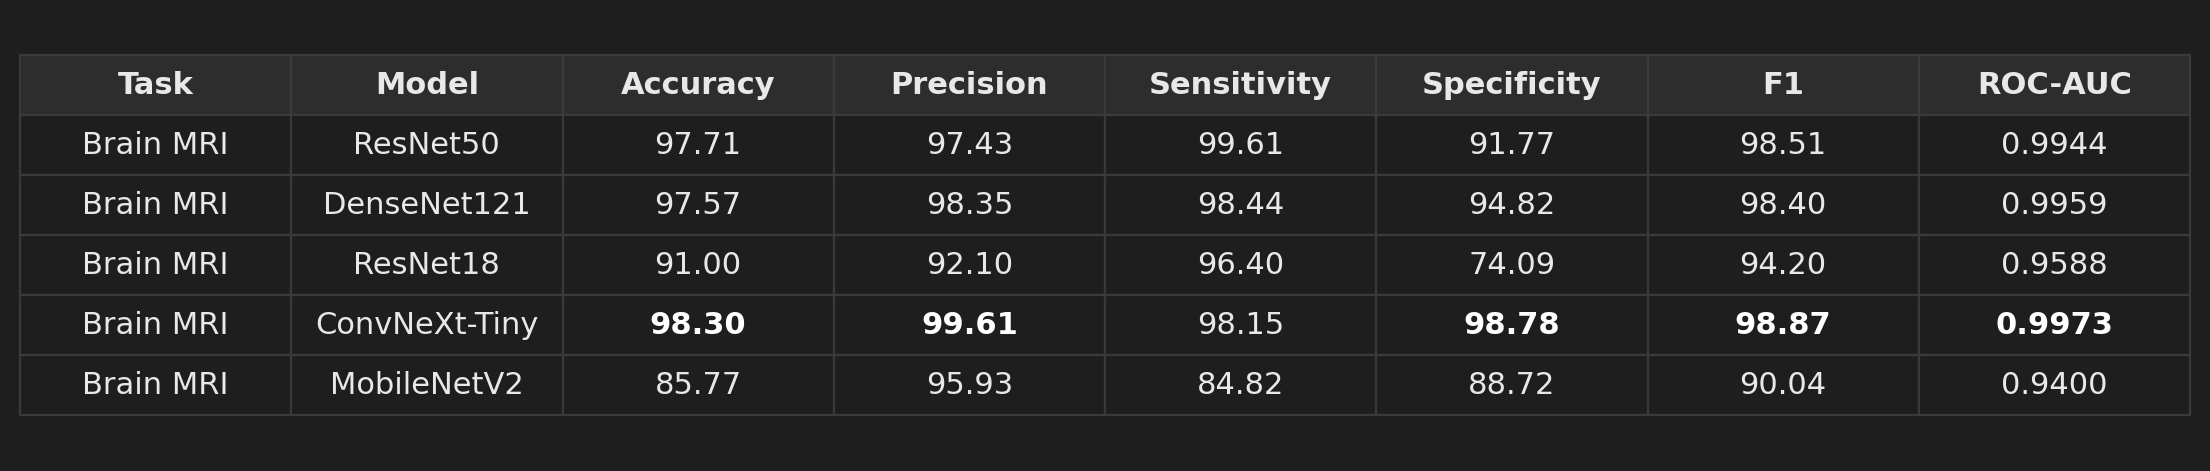
\includegraphics[width=\linewidth]{paper_tables/brain_tumor_mri/table03_clean_brain_mri_five_models.png}
  \caption{Clean image classification performance on Brain MRI ($n=1356$).}
  \label{fig:brain_mri_clean_five_models}
\end{figure}

\begin{figure}[htbp]
  \centering
  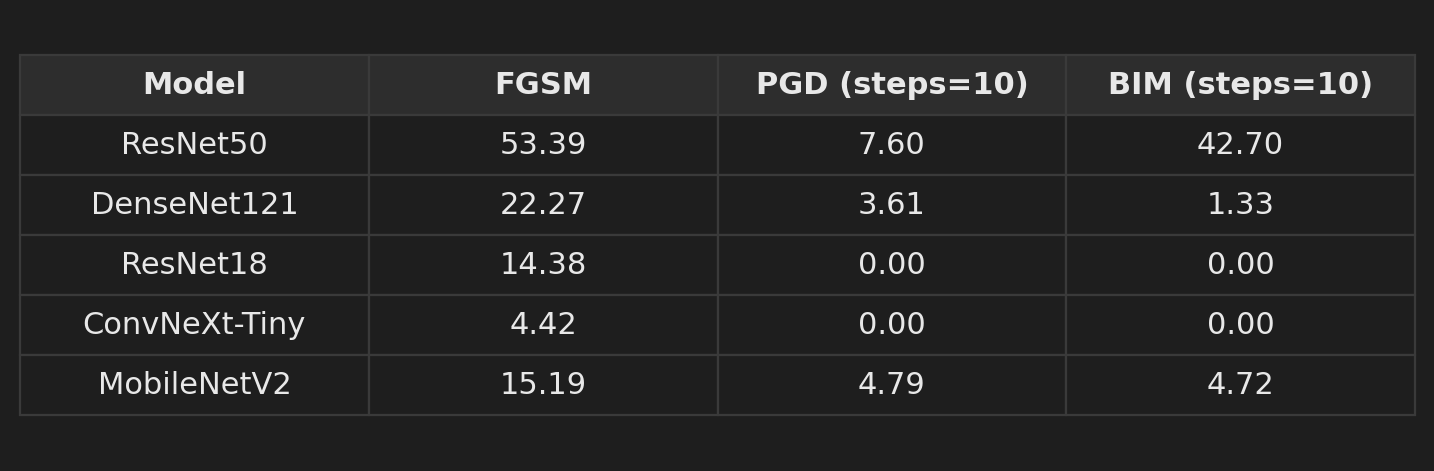
\includegraphics[width=0.85\linewidth]{paper_tables/brain_tumor_mri/table04_robustness_five_models_eps4.png}
  \caption{Adversarial accuracy (\%) of five standard models on Brain MRI at $\epsilon=4/255$.}
  \label{fig:brain_mri_robustness_eps4}
\end{figure}

\begin{figure}[htbp]
  \centering
  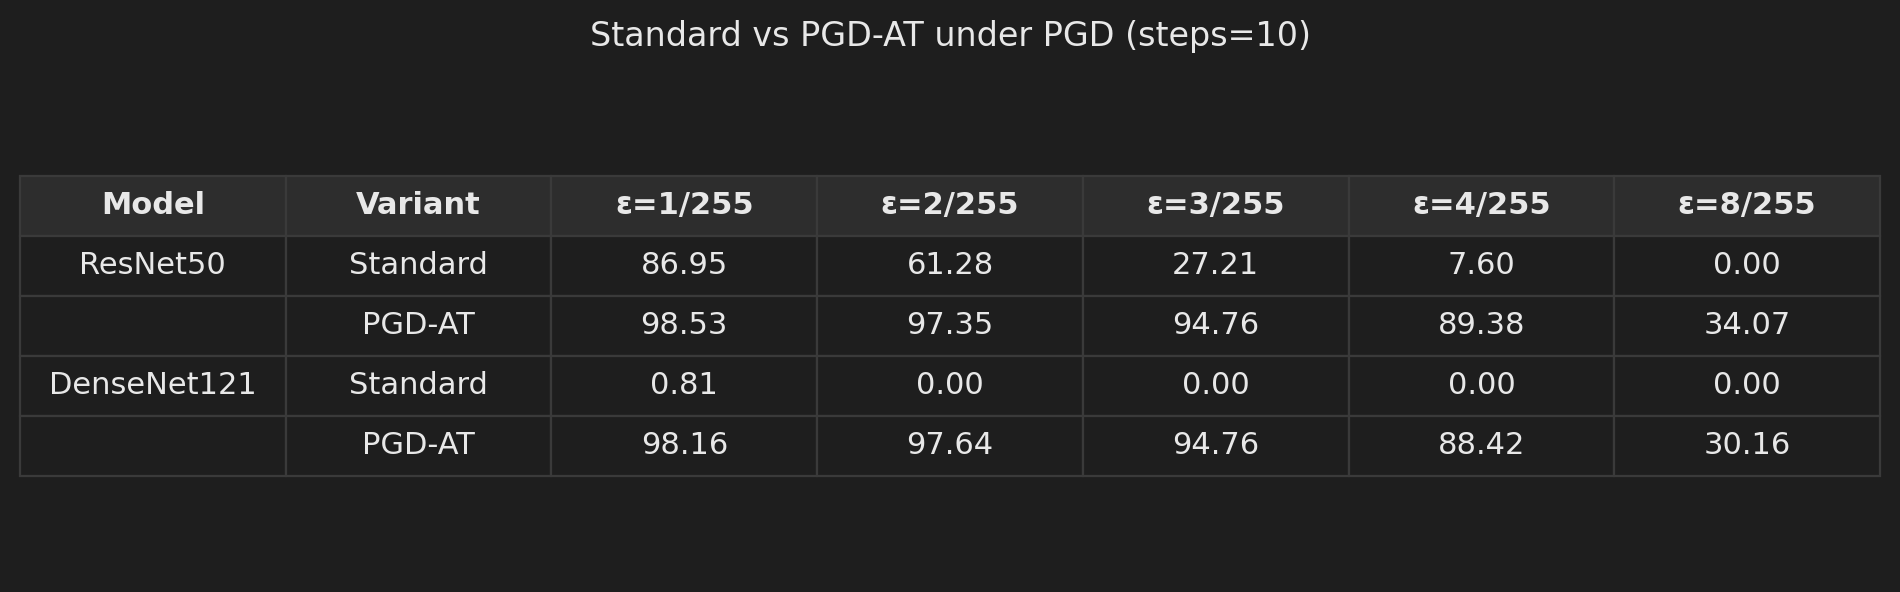
\includegraphics[width=\linewidth]{paper_tables/brain_tumor_mri/table05_pgd_at_pgd_attack_steps10.png}
  \caption{Standard vs.\ PGD-AT accuracy (\%) under PGD attack (steps=10) on Brain MRI.}
  \label{fig:pgd_at_pgd_steps10}
\end{figure}

\begin{figure}[htbp]
  \centering
  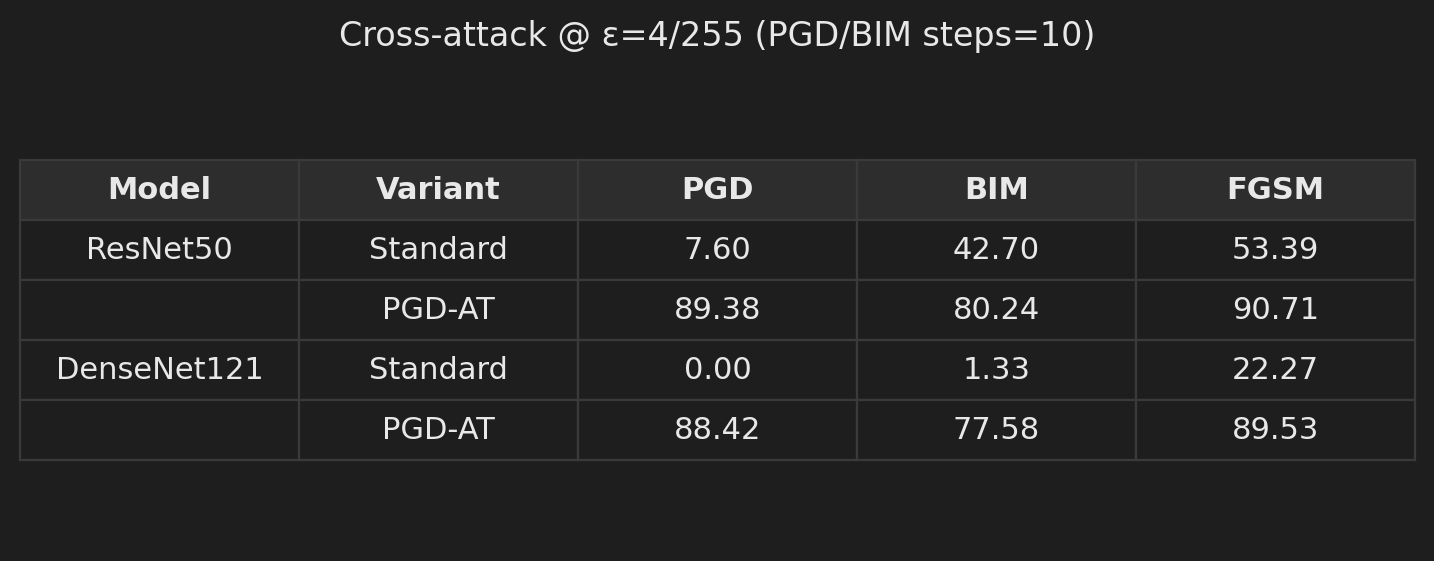
\includegraphics[width=0.85\linewidth]{paper_tables/brain_tumor_mri/table06_pgd_at_cross_attack_eps4.png}
  \caption{Standard vs.\ PGD-AT accuracy (\%) under three attacks at $\epsilon=4/255$ (Brain MRI).}
  \label{fig:pgd_at_cross_attack_eps4}
\end{figure}

\begin{figure}[htbp]
  \centering
  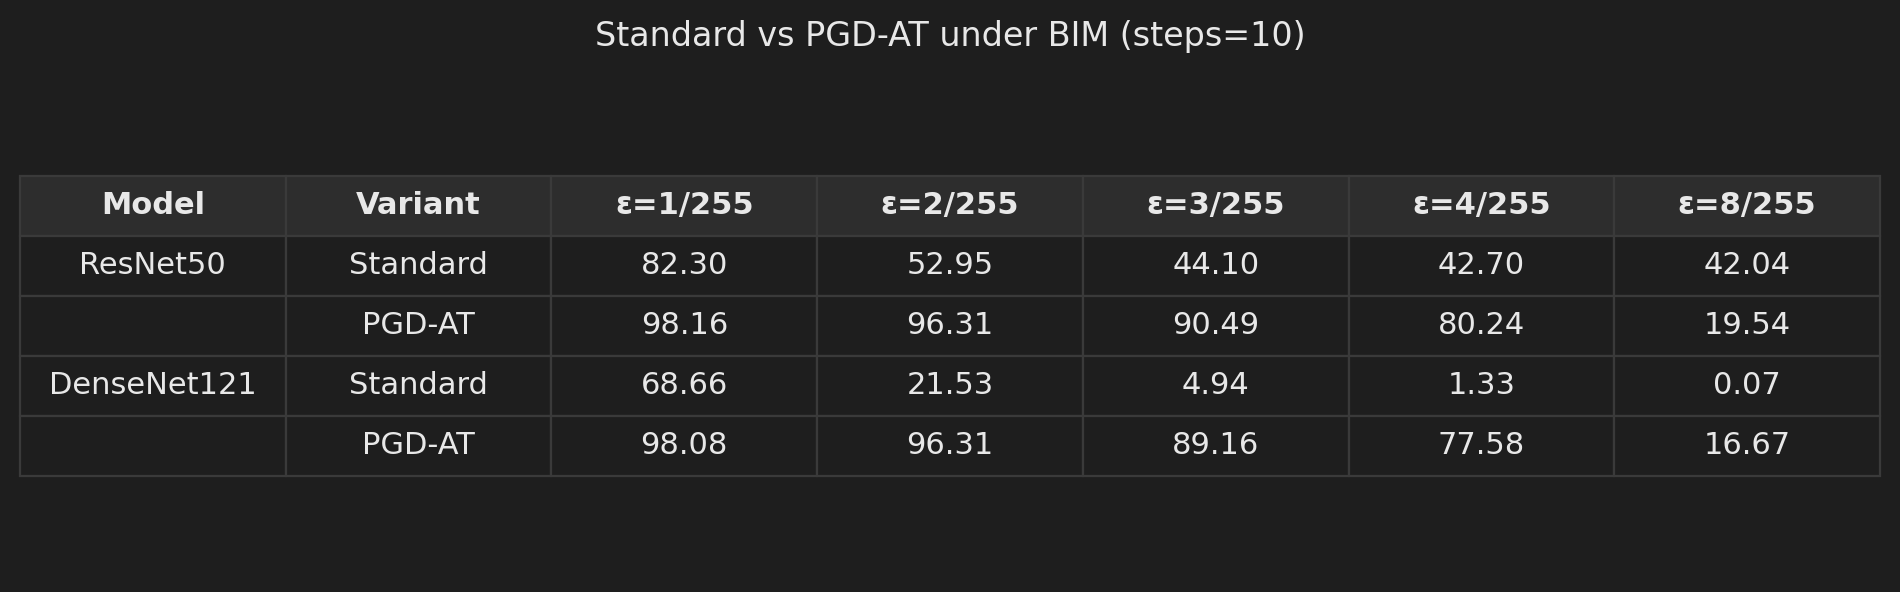
\includegraphics[width=\linewidth]{paper_tables/brain_tumor_mri/table07_pgd_at_bim_steps10.png}
  \caption{Standard vs.\ PGD-AT accuracy (\%) under BIM attack (steps=10) on Brain MRI.}
  \label{fig:pgd_at_bim_steps10}
\end{figure}

\begin{figure}[htbp]
  \centering
  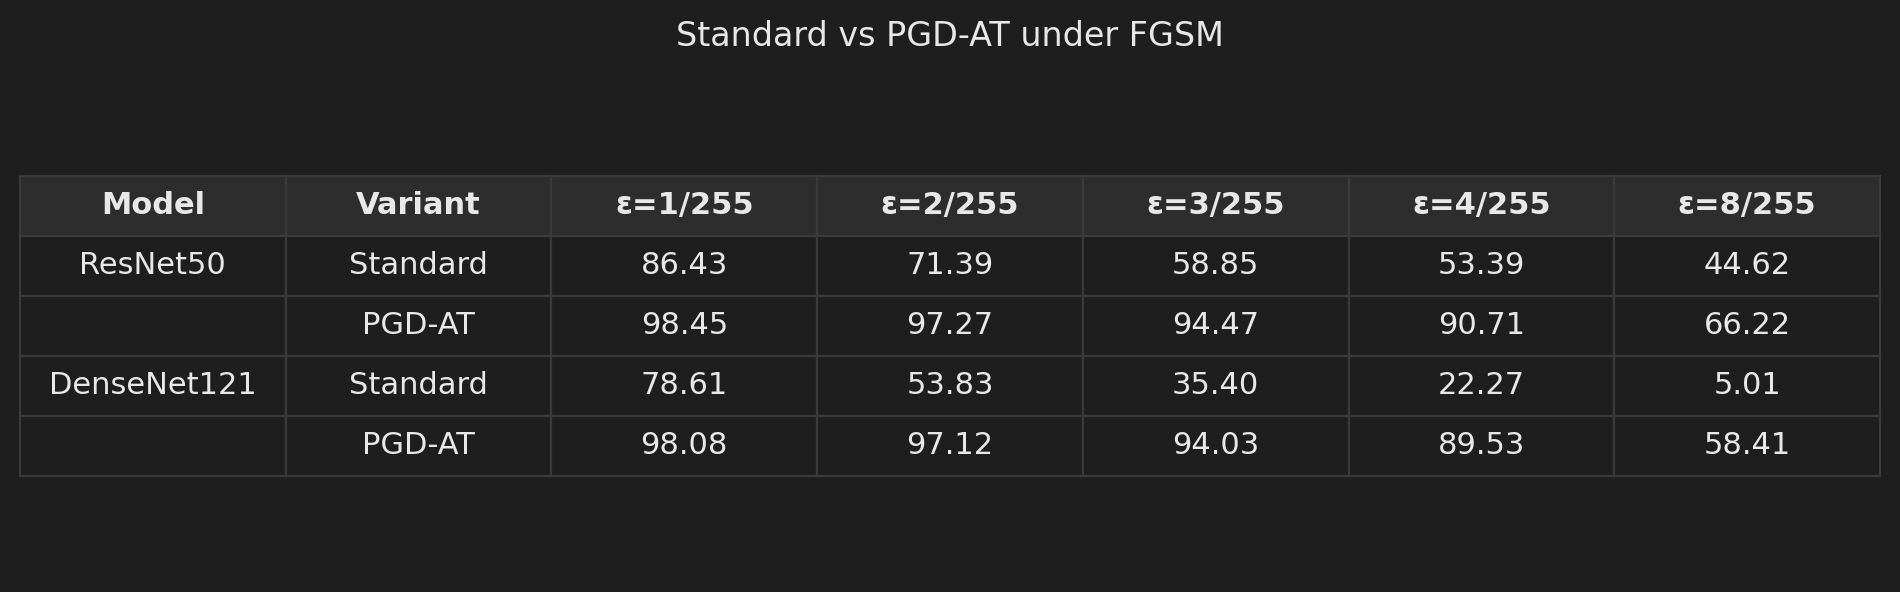
\includegraphics[width=\linewidth]{paper_tables/brain_tumor_mri/table08_pgd_at_fgsm.png}
  \caption{Standard vs.\ PGD-AT accuracy (\%) under FGSM attack on Brain MRI.}
  \label{fig:pgd_at_fgsm}
\end{figure}


\begin{figure}[htbp]
  \centering
  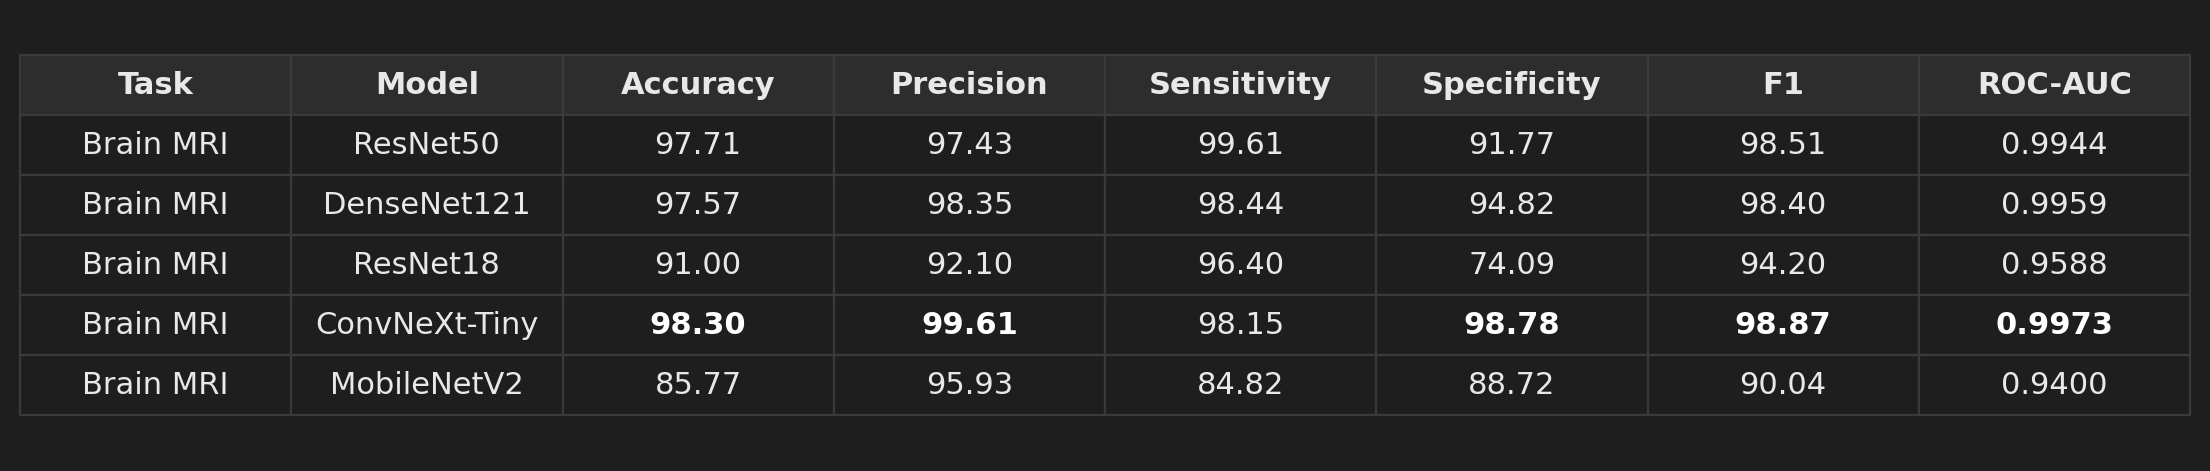
\includegraphics[width=\linewidth]{paper_tables/brain_tumor_mri/table03_clean_brain_mri_five_models.png}
  \caption{Clean image classification performance on Brain MRI ($n=1356$).}
  \label{fig:brain_mri_clean_five_models}
\end{figure}

\begin{figure}[htbp]
  \centering
  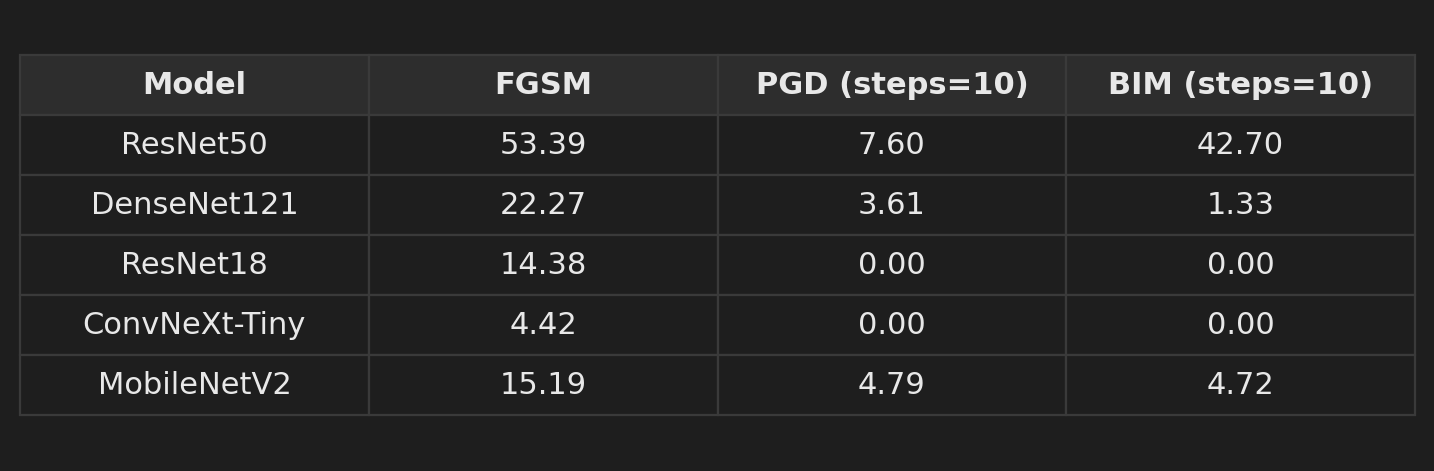
\includegraphics[width=0.85\linewidth]{paper_tables/brain_tumor_mri/table04_robustness_five_models_eps4.png}
  \caption{Adversarial accuracy (\%) of five standard models on Brain MRI at $\epsilon=4/255$.}
  \label{fig:brain_mri_robustness_eps4}
\end{figure}

\begin{figure}[htbp]
  \centering
  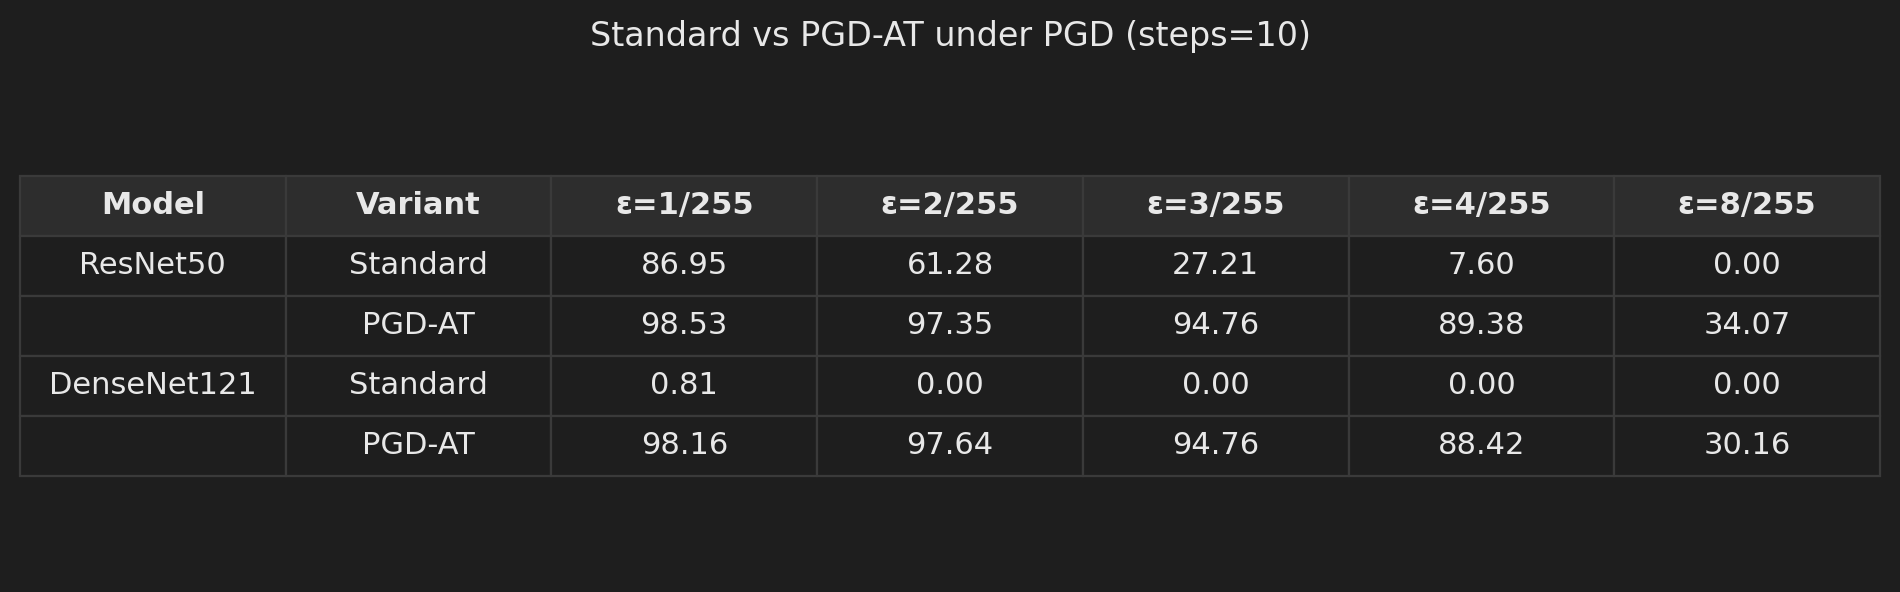
\includegraphics[width=\linewidth]{paper_tables/brain_tumor_mri/table05_pgd_at_pgd_attack_steps10.png}
  \caption{Standard vs.\ PGD-AT accuracy (\%) under PGD attack (steps=10) on Brain MRI.}
  \label{fig:pgd_at_pgd_steps10}
\end{figure}

\begin{figure}[htbp]
  \centering
  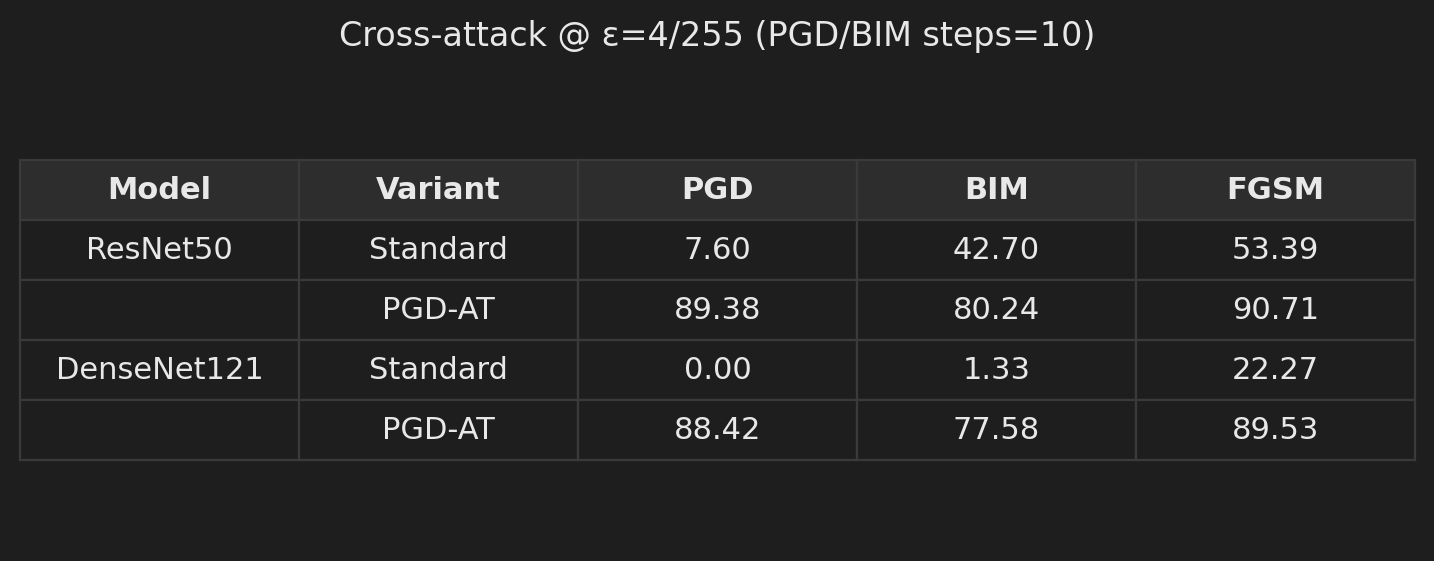
\includegraphics[width=0.85\linewidth]{paper_tables/brain_tumor_mri/table06_pgd_at_cross_attack_eps4.png}
  \caption{Standard vs.\ PGD-AT accuracy (\%) under three attacks at $\epsilon=4/255$ (Brain MRI).}
  \label{fig:pgd_at_cross_attack_eps4}
\end{figure}

\begin{figure}[htbp]
  \centering
  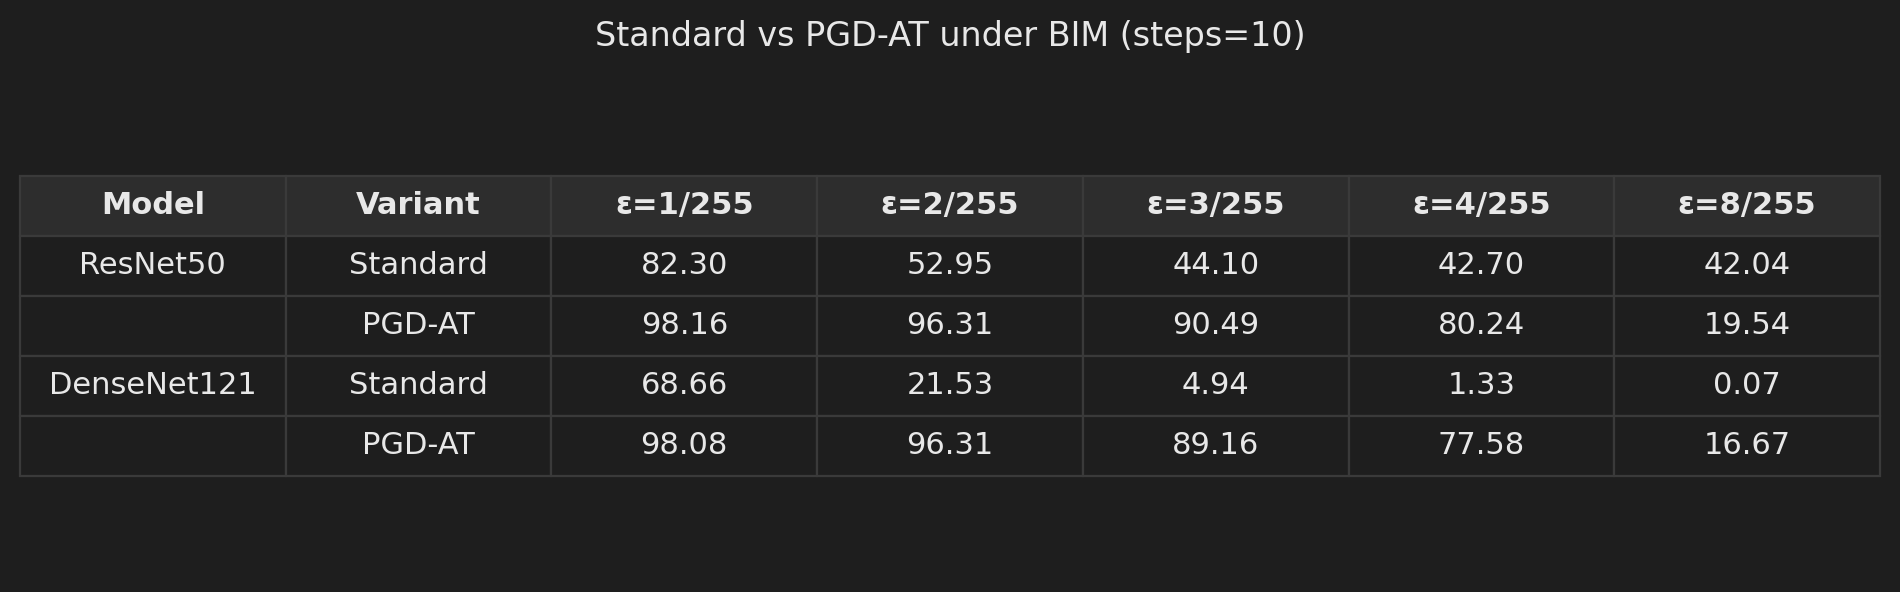
\includegraphics[width=\linewidth]{paper_tables/brain_tumor_mri/table07_pgd_at_bim_steps10.png}
  \caption{Standard vs.\ PGD-AT accuracy (\%) under BIM attack (steps=10) on Brain MRI.}
  \label{fig:pgd_at_bim_steps10}
\end{figure}

\begin{figure}[htbp]
  \centering
  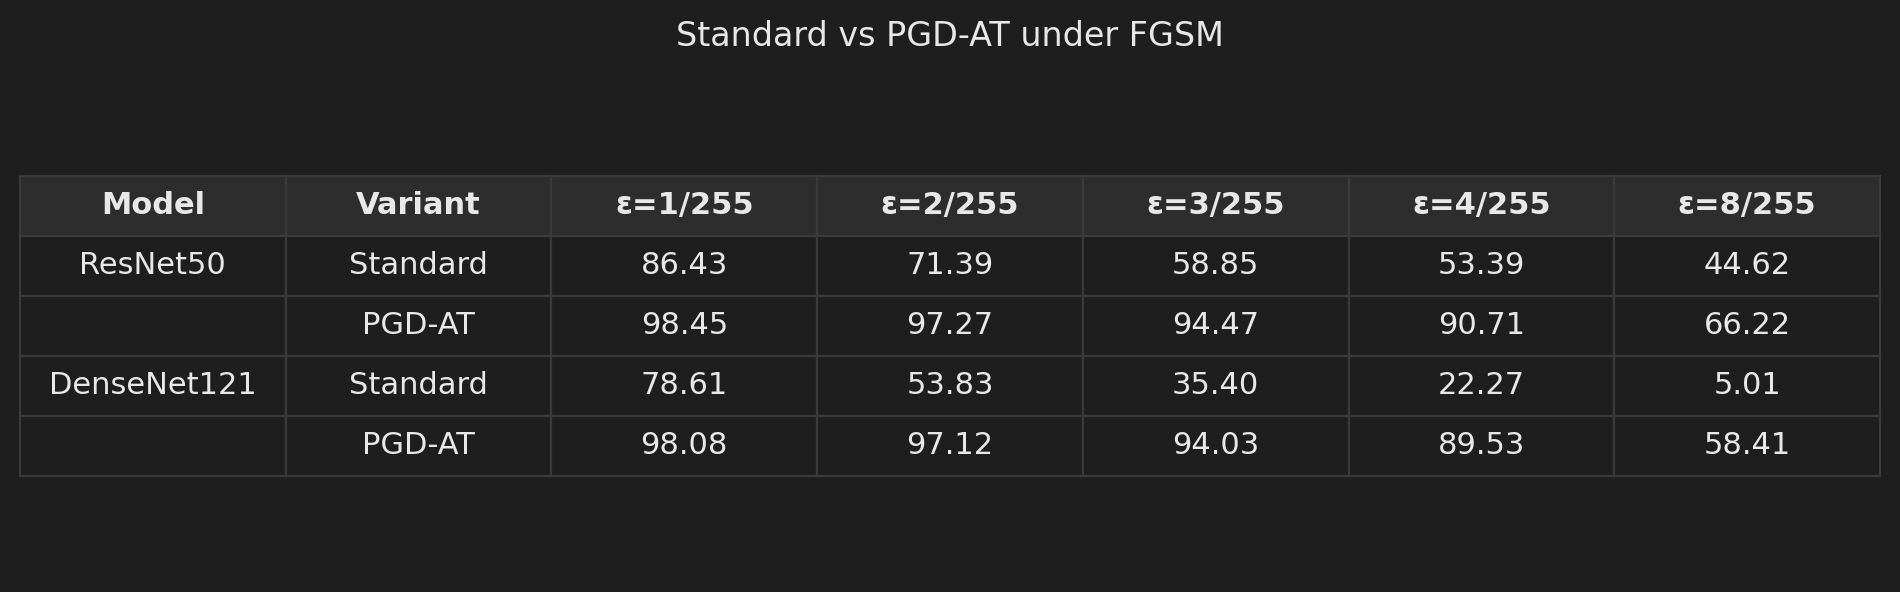
\includegraphics[width=\linewidth]{paper_tables/brain_tumor_mri/table08_pgd_at_fgsm.png}
  \caption{Standard vs.\ PGD-AT accuracy (\%) under FGSM attack on Brain MRI.}
  \label{fig:pgd_at_fgsm}
\end{figure}


\begin{figure}[htbp]
  \centering
  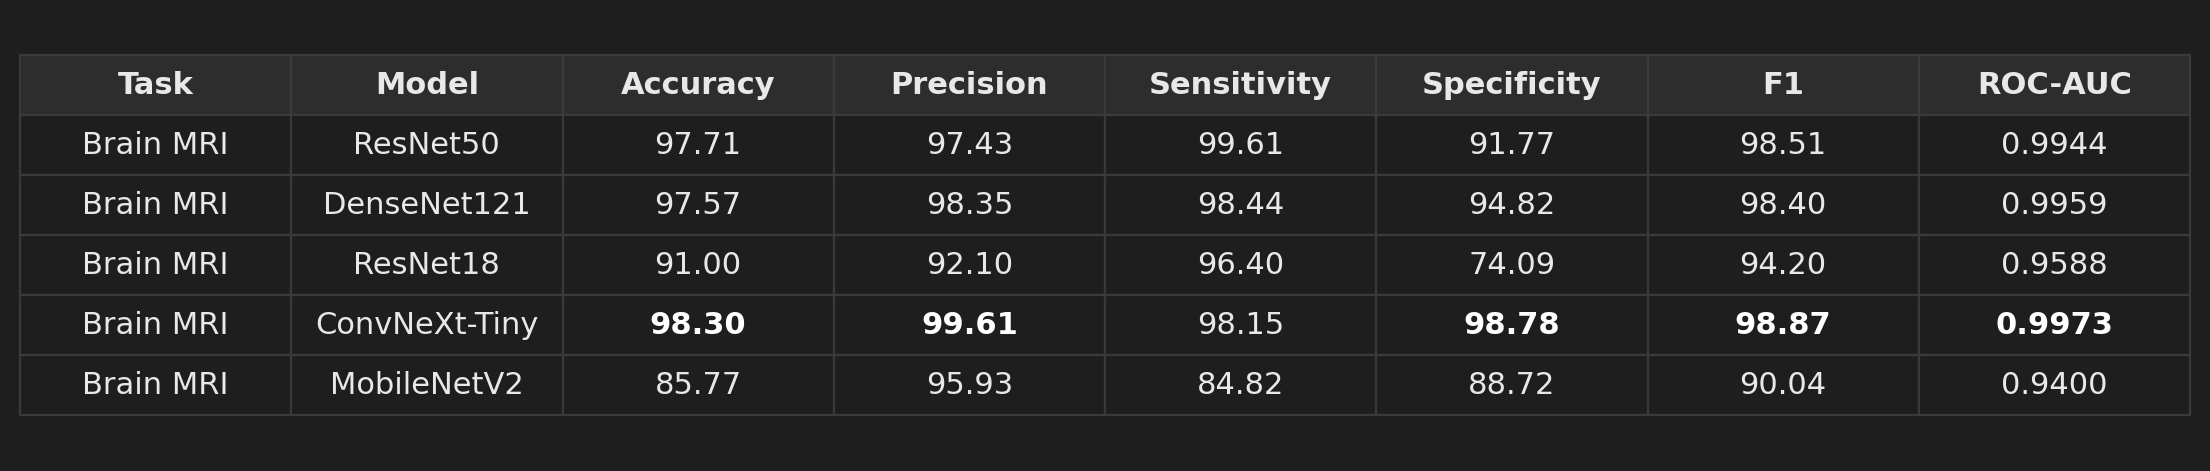
\includegraphics[width=\linewidth]{paper_tables/brain_tumor_mri/table03_clean_brain_mri_five_models.png}
  \caption{Clean image classification performance on Brain MRI ($n=1356$).}
  \label{fig:brain_mri_clean_five_models}
\end{figure}

\begin{figure}[htbp]
  \centering
  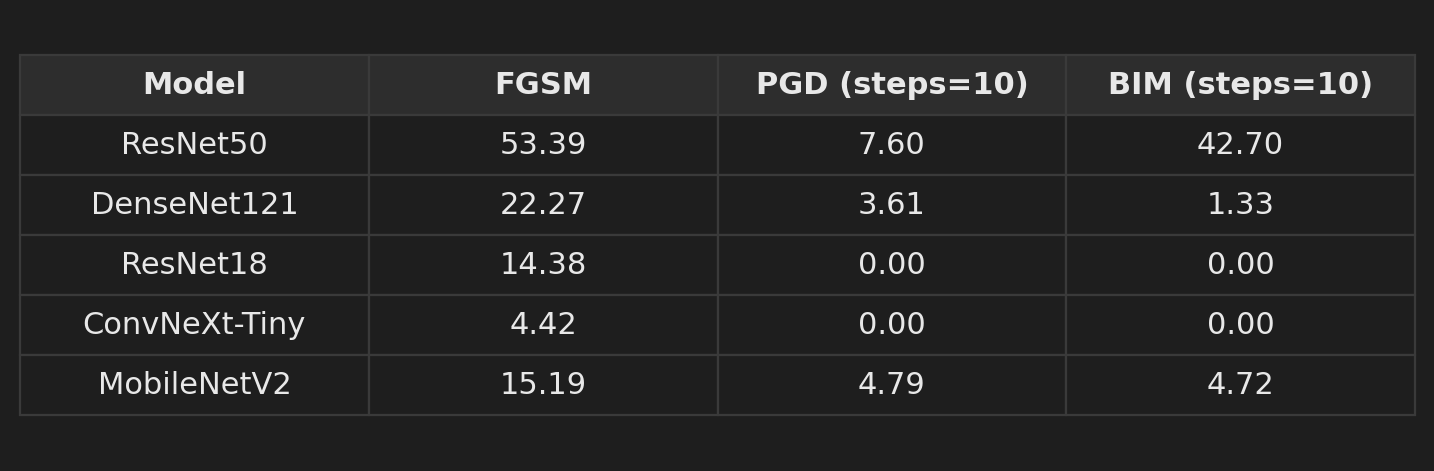
\includegraphics[width=0.85\linewidth]{paper_tables/brain_tumor_mri/table04_robustness_five_models_eps4.png}
  \caption{Adversarial accuracy (\%) of five standard models on Brain MRI at $\epsilon=4/255$.}
  \label{fig:brain_mri_robustness_eps4}
\end{figure}

\begin{figure}[htbp]
  \centering
  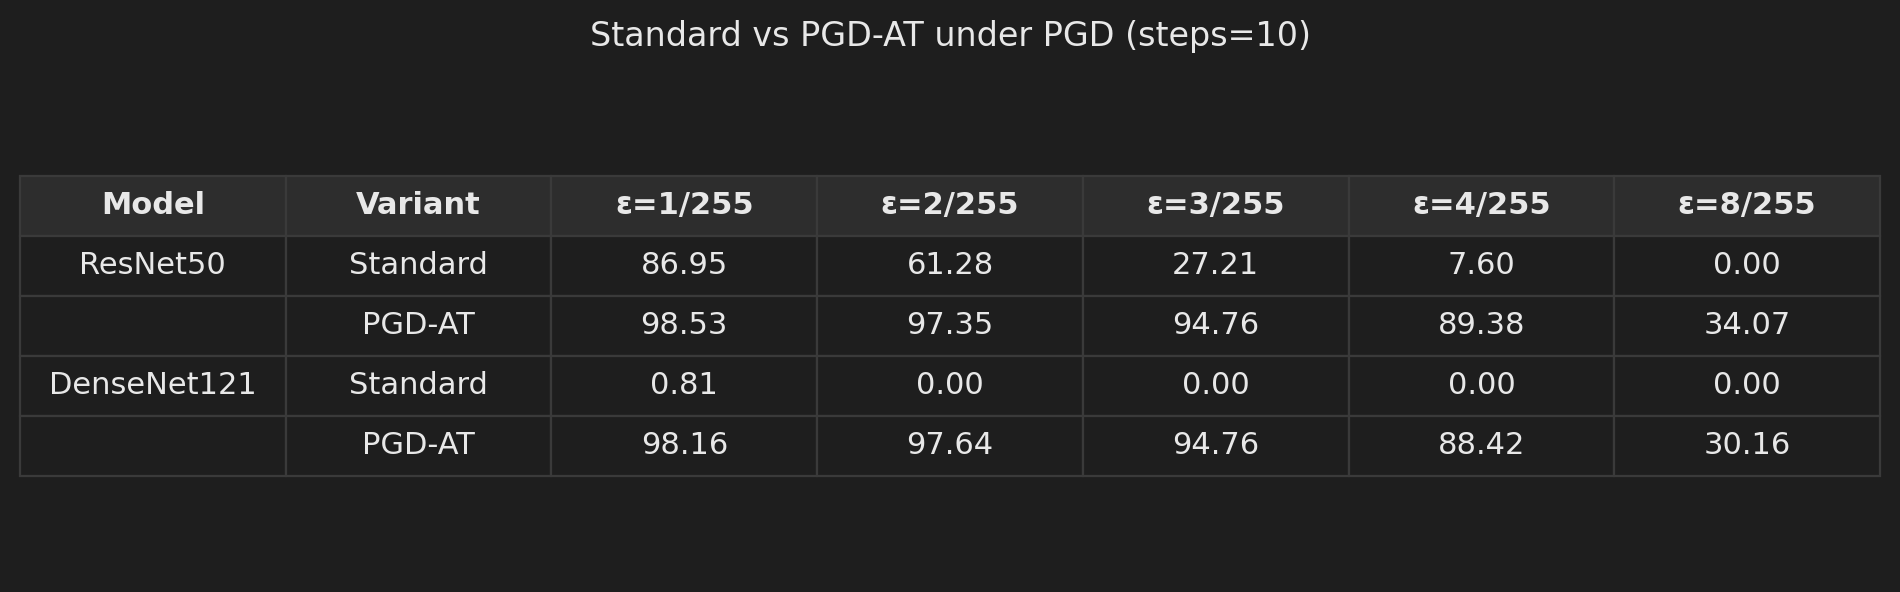
\includegraphics[width=\linewidth]{paper_tables/brain_tumor_mri/table05_pgd_at_pgd_attack_steps10.png}
  \caption{Standard vs.\ PGD-AT accuracy (\%) under PGD attack (steps=10) on Brain MRI.}
  \label{fig:pgd_at_pgd_steps10}
\end{figure}

\begin{figure}[htbp]
  \centering
  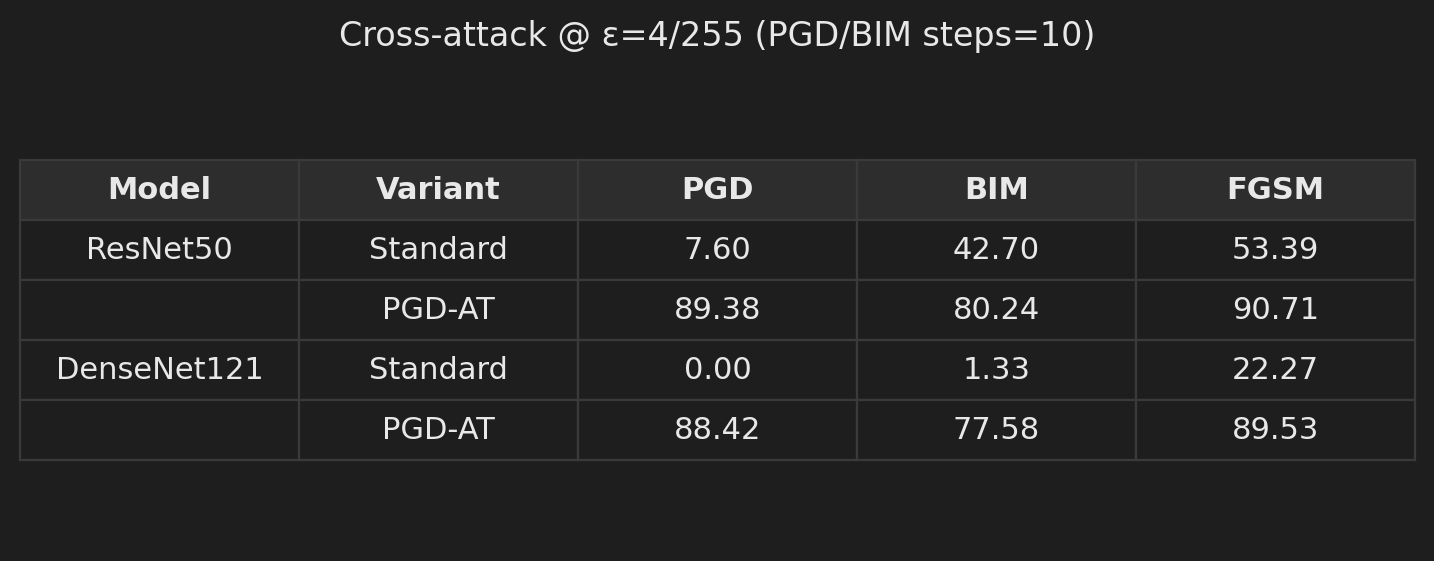
\includegraphics[width=0.85\linewidth]{paper_tables/brain_tumor_mri/table06_pgd_at_cross_attack_eps4.png}
  \caption{Standard vs.\ PGD-AT accuracy (\%) under three attacks at $\epsilon=4/255$ (Brain MRI).}
  \label{fig:pgd_at_cross_attack_eps4}
\end{figure}

\begin{figure}[htbp]
  \centering
  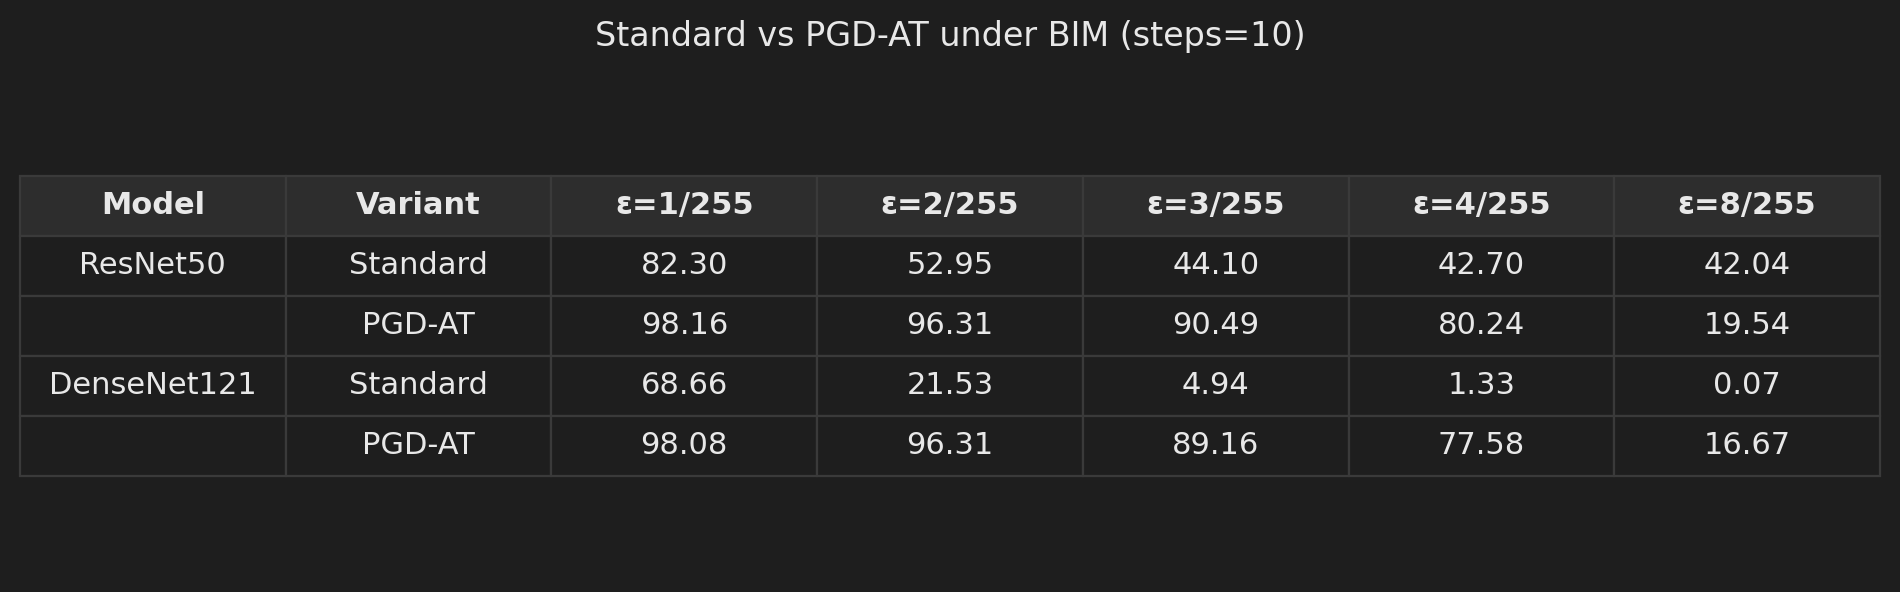
\includegraphics[width=\linewidth]{paper_tables/brain_tumor_mri/table07_pgd_at_bim_steps10.png}
  \caption{Standard vs.\ PGD-AT accuracy (\%) under BIM attack (steps=10) on Brain MRI.}
  \label{fig:pgd_at_bim_steps10}
\end{figure}

\begin{figure}[htbp]
  \centering
  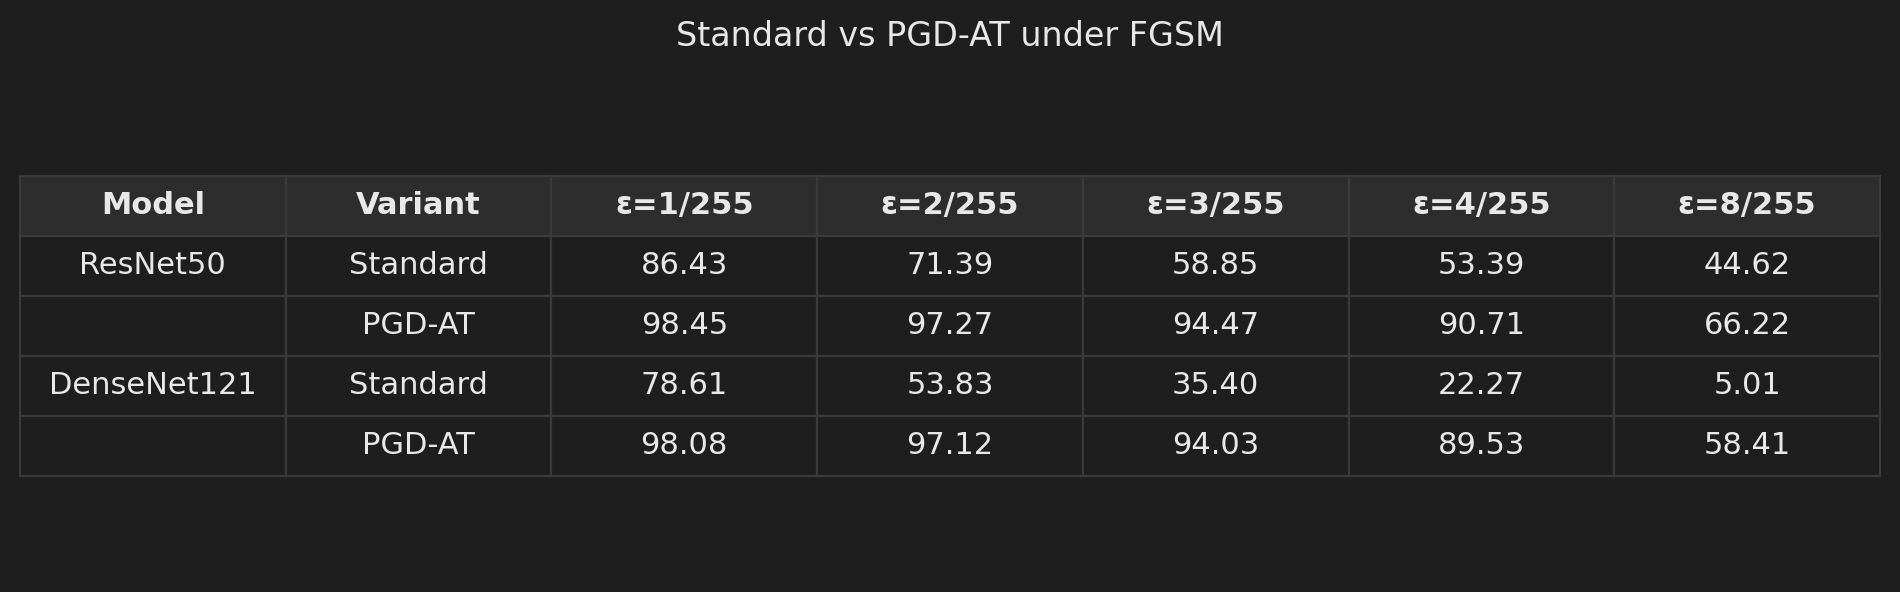
\includegraphics[width=\linewidth]{paper_tables/brain_tumor_mri/table08_pgd_at_fgsm.png}
  \caption{Standard vs.\ PGD-AT accuracy (\%) under FGSM attack on Brain MRI.}
  \label{fig:pgd_at_fgsm}
\end{figure}


\begin{figure}[htbp]
  \centering
  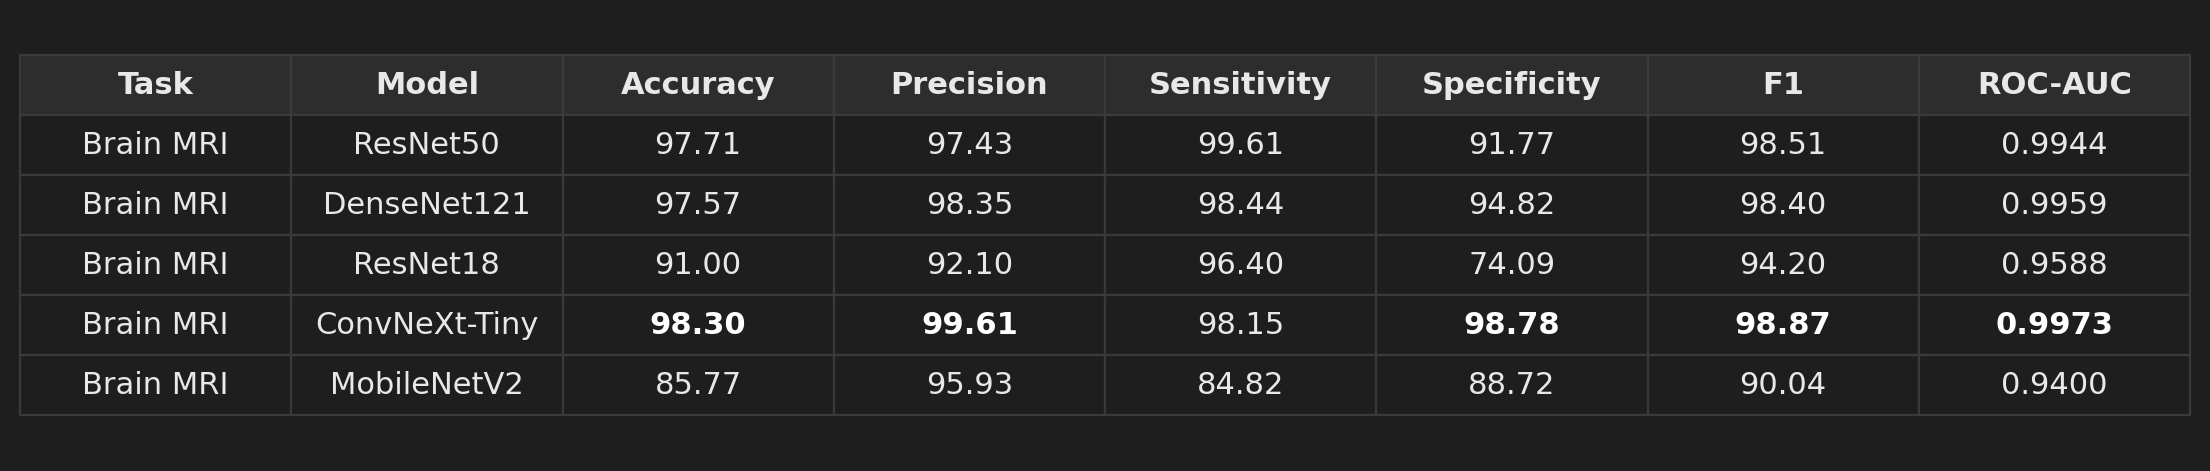
\includegraphics[width=\linewidth]{paper_tables/brain_tumor_mri/table03_clean_brain_mri_five_models.png}
  \caption{Clean image classification performance on Brain MRI ($n=1356$).}
  \label{fig:brain_mri_clean_five_models}
\end{figure}

\begin{figure}[htbp]
  \centering
  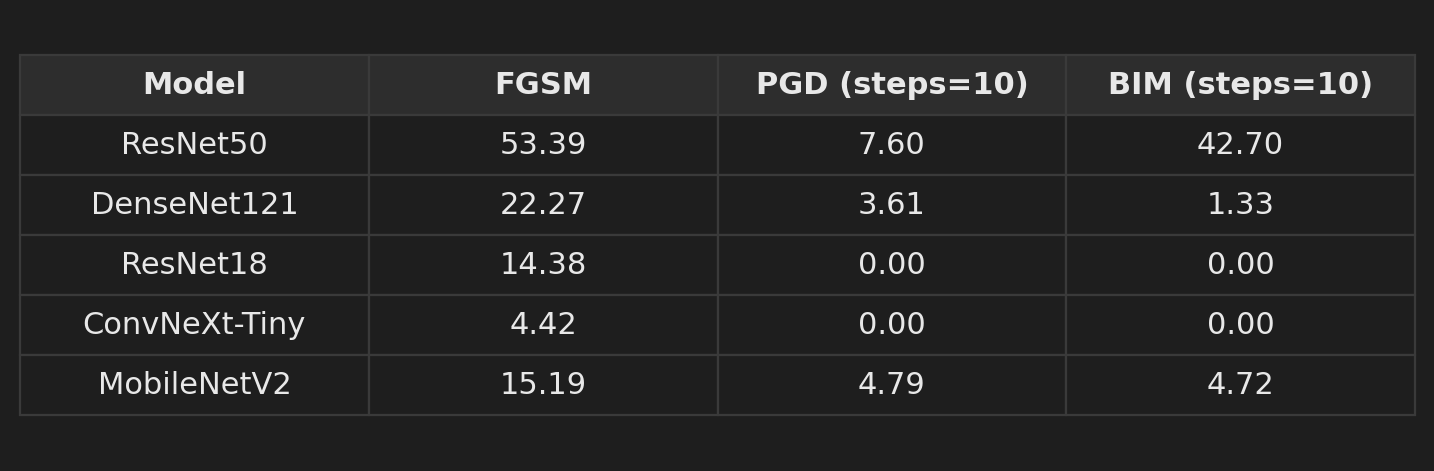
\includegraphics[width=0.85\linewidth]{paper_tables/brain_tumor_mri/table04_robustness_five_models_eps4.png}
  \caption{Adversarial accuracy (\%) of five standard models on Brain MRI at $\epsilon=4/255$.}
  \label{fig:brain_mri_robustness_eps4}
\end{figure}

\begin{figure}[htbp]
  \centering
  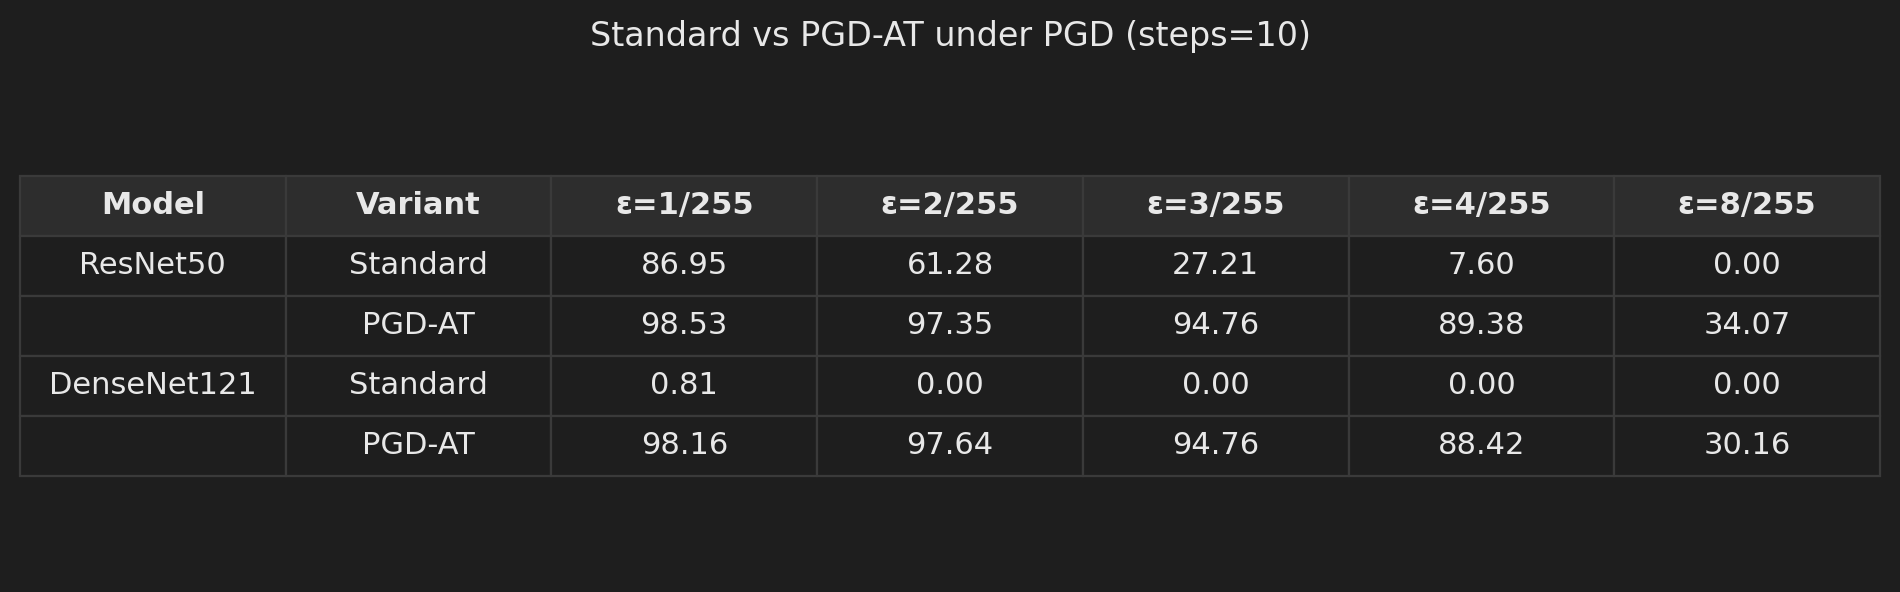
\includegraphics[width=\linewidth]{paper_tables/brain_tumor_mri/table05_pgd_at_pgd_attack_steps10.png}
  \caption{Standard vs.\ PGD-AT accuracy (\%) under PGD attack (steps=10) on Brain MRI.}
  \label{fig:pgd_at_pgd_steps10}
\end{figure}

\begin{figure}[htbp]
  \centering
  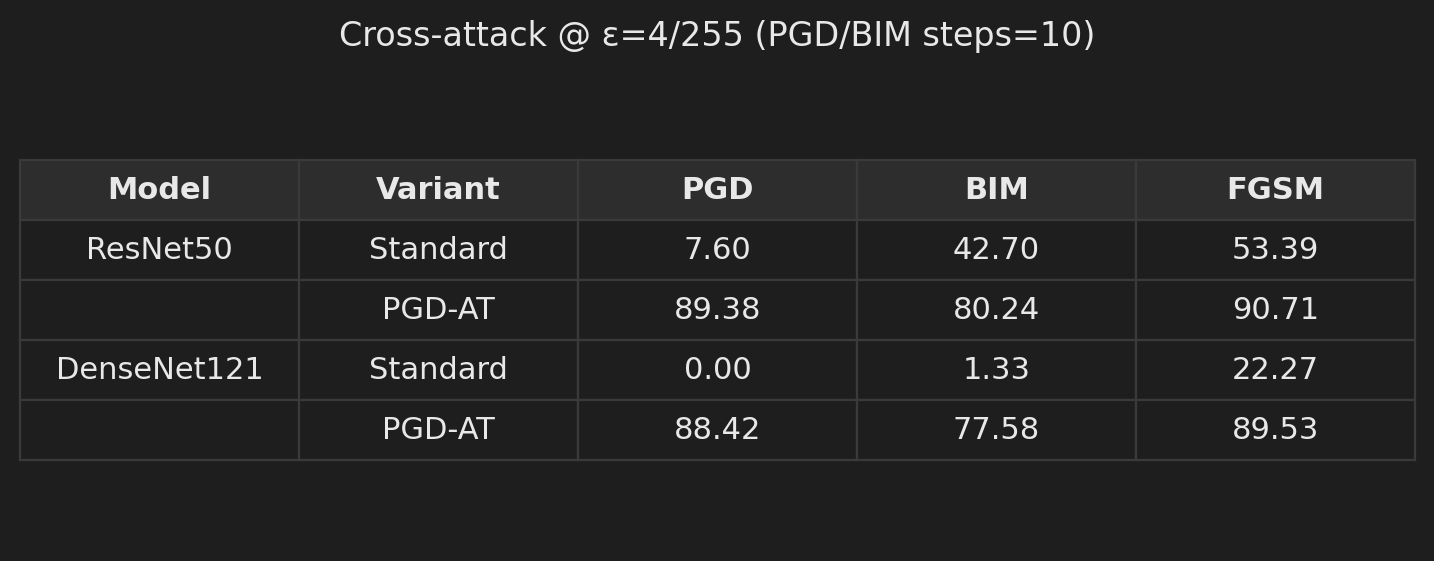
\includegraphics[width=0.85\linewidth]{paper_tables/brain_tumor_mri/table06_pgd_at_cross_attack_eps4.png}
  \caption{Standard vs.\ PGD-AT accuracy (\%) under three attacks at $\epsilon=4/255$ (Brain MRI).}
  \label{fig:pgd_at_cross_attack_eps4}
\end{figure}

\begin{figure}[htbp]
  \centering
  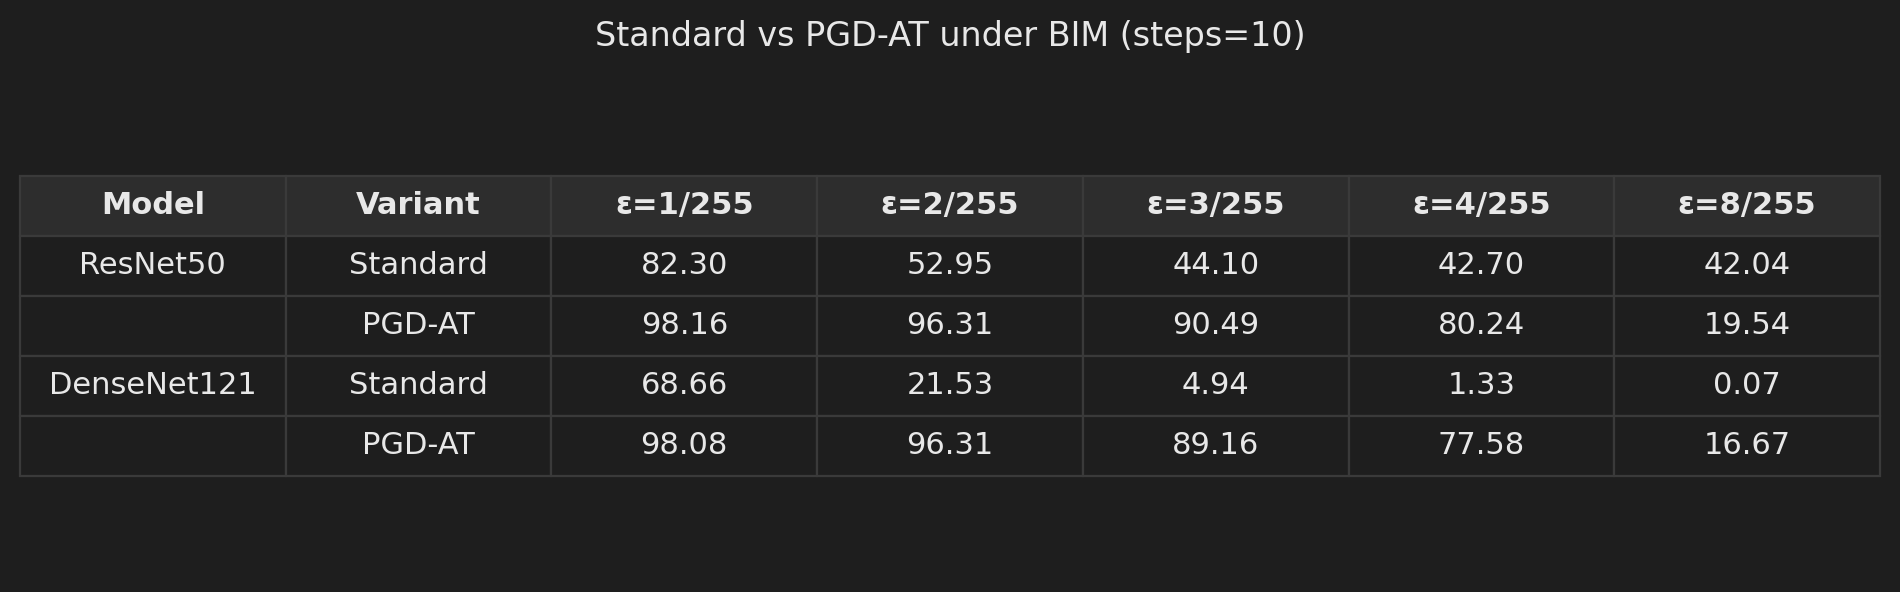
\includegraphics[width=\linewidth]{paper_tables/brain_tumor_mri/table07_pgd_at_bim_steps10.png}
  \caption{Standard vs.\ PGD-AT accuracy (\%) under BIM attack (steps=10) on Brain MRI.}
  \label{fig:pgd_at_bim_steps10}
\end{figure}

\begin{figure}[htbp]
  \centering
  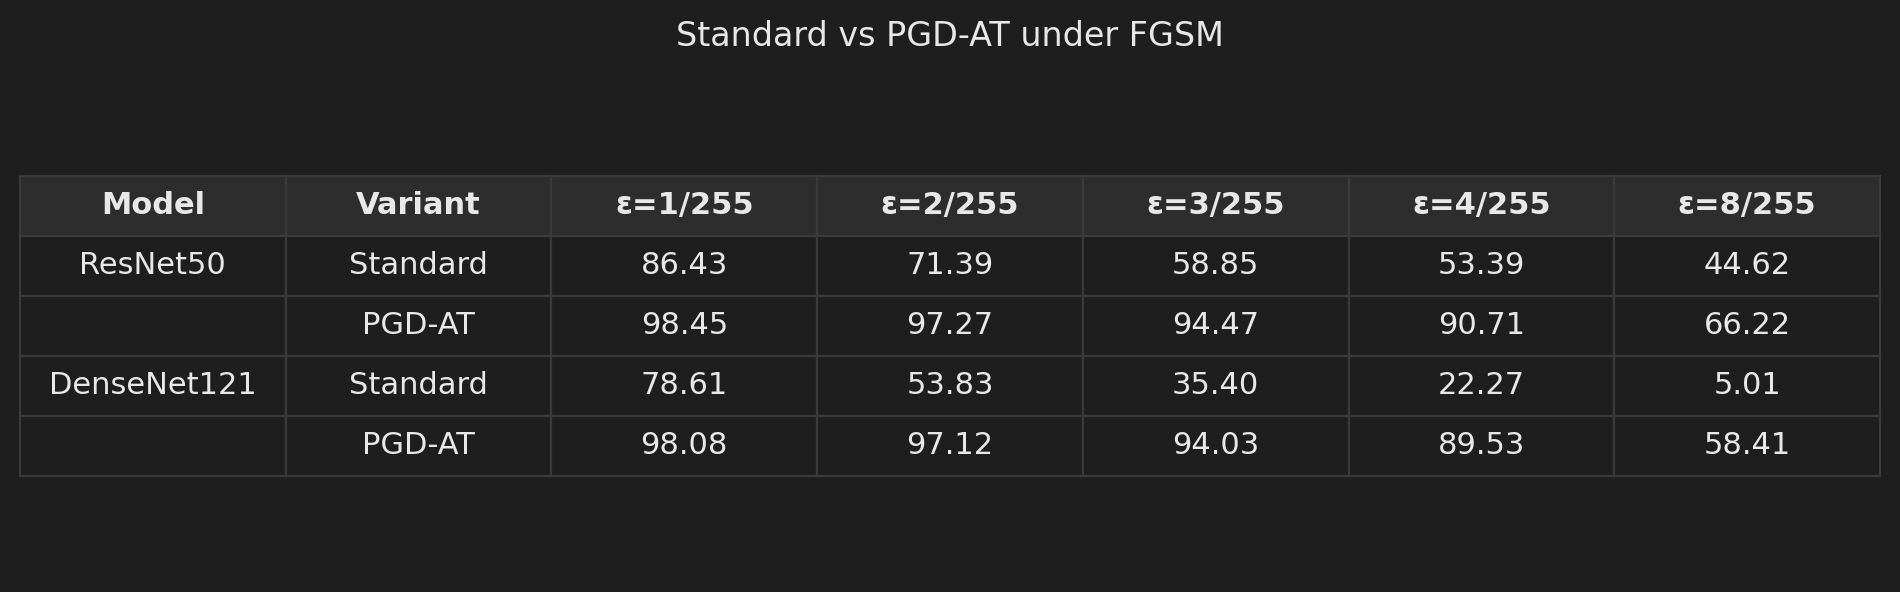
\includegraphics[width=\linewidth]{paper_tables/brain_tumor_mri/table08_pgd_at_fgsm.png}
  \caption{Standard vs.\ PGD-AT accuracy (\%) under FGSM attack on Brain MRI.}
  \label{fig:pgd_at_fgsm}
\end{figure}
